% Revised and extended version of Chauhan & Hegde, DATA 2026, for Springer CCIS.
% Build: pdflatex main && bibtex main && pdflatex main && pdflatex main
\documentclass[runningheads]{llncs}
\usepackage[T1]{fontenc}
\usepackage{newtxtext}
\usepackage[varvw]{newtxmath}
\usepackage{graphicx}
\usepackage{booktabs}
\usepackage{multirow}
\usepackage{url}
\usepackage{color}
\renewcommand\UrlFont{\color{blue}\rmfamily}
\urlstyle{rm}

% \tbd{} marks any remaining placeholder (should be none at submission)
\newcommand{\tbd}[1]{\textbf{[TBD: #1]}}

\begin{document}

\title{When Does Chunking Matter? A Three-Regime Variance Decomposition of Segmentation Effects in Retrieval-Augmented Generation\thanks{This paper is a revised and extended version of ``Chunking Is Not the Bottleneck: Why RAG Evaluation Must Look Beyond Segmentation Strategy'' presented at DATA 2026~\cite{chauhan2026chunking}. See Sect.~\ref{sec:whatsnew} for a summary of the extensions. This chapter was prepared with the assistance of AI; see the disclosure at the end of the chapter for details.}}
\titlerunning{When Does Chunking Matter?}

\author{Aaditya Chauhan\inst{1}\orcidID{0009-0000-8652-0071} \and
Nivas Hegde\inst{1}\orcidID{0009-0007-2895-6644}}
\authorrunning{A. Chauhan and N. Hegde}
\institute{Independent Researcher, U.S.A.\\
\email{aadityc28@gmail.com}, \email{nivas25h@gmail.com}}
% TODO: mark exactly one corresponding author (Springer requires it) and confirm affiliation wording.

\maketitle

\begin{abstract}
Practitioners building retrieval-augmented generation (RAG) systems devote considerable effort to choosing a text-chunking strategy. In earlier work we showed, with a balanced factorial experiment on Natural Questions and MS-MARCO, that chunking strategy explains only 1--2\% of the variance in retrieval quality and is not statistically significant, whereas dataset identity and embedding model together explain 67--89\%. This article asks the natural follow-up question: \emph{when} does chunking matter? We repeat the same variance-decomposition design on two further corpus regimes with rigorous gold labels: 24 structured technical documents spanning eight domains (576 configurations), and the four long-contract sub-benchmarks of LegalBench-RAG with expert-annotated character spans (144 configurations), adding a third embedding model throughout. Chunking's share of variance is regime-dependent and non-monotonic: it rises to 5--8\% and becomes highly significant on technical documentation, then falls below 1\% on long legal contracts. A strategy-by-regime interaction explains 12--20\% of variance. Across all 28 corpora, the density of explicit section headings predicts the size of the chunking effect ($\rho = 0.58$), whereas document length does not. A legal-aware structure parser that detects section structure in 72\% of contracts does not rescue structure-aware chunking there, and a boundary-versus-metadata ablation shows that where structure-aware chunking helps, the heading-path prefix accounts for most of the end-to-end gain. We argue that RAG benchmarks should report variance decomposition and interaction effects alongside absolute scores, and we give practitioners a simple diagnostic for deciding whether chunking deserves engineering attention on their corpus.

\keywords{Retrieval-augmented generation \and Text chunking \and Variance decomposition \and Benchmark evaluation \and Embedding models \and Legal document retrieval.}
\end{abstract}

\section{Introduction}
\label{sec:intro}

Retrieval-augmented generation (RAG) grounds a large language model (LLM) in external documents by retrieving passages at query time and placing them in the model's context~\cite{lewis2020rag,gao2023survey}. Before anything can be retrieved, documents must be segmented into retrieval units, and this chunking step has become one of the most discussed design decisions in the RAG ecosystem. Framework documentation~\cite{langchain2023,llamaindex2023}, tutorials~\cite{kamradt2023}, and a growing body of papers~\cite{jimenoyepes2024financial,qu2025semantic,duarte2024lumberchunker,zhao2024metachunking} compare fixed-size, sentence-based, recursive, semantic, and structure-aware splitters, and the engineering folklore holds that getting chunk boundaries right is essential.

In the conference version of this work~\cite{chauhan2026chunking} we tested that folklore with a controlled experiment. Crossing four chunking strategies, two embedding models, two chunk sizes and two established question-answering (QA) datasets, and decomposing the variance of six retrieval metrics with a Type III analysis of variance (ANOVA), we found that chunking strategy accounted for only 1--2\% of total variance and was not statistically significant, while dataset identity (24--78\%) and embedding model (11--50\%) dominated. An end-to-end evaluation with an LLM judge showed that the small retrieval differences did not propagate to answer quality. We concluded that, for factoid QA over general-purpose natural-language corpora, chunking is a low-variance factor and that the community's attention to it was disproportionate.

That conclusion was deliberately bounded. The conference paper listed settings in which chunking might matter more, including very long documents, strongly structured content, and non-QA tasks, but tested none of them. Several studies published since then make the question urgent, because they disagree with one another: some report that simple chunking is sufficient~\cite{bennani2026systematic,caspari2026complex,kreileder2026academic,li2025enhancing}, while others report that the right chunker nearly doubles retrieval quality~\cite{shaukat2026systematic} or dominates retrieval gains on legal contracts~\cite{singh2026strucchunk}. Absolute metric comparisons on different corpora cannot resolve this disagreement. A variance decomposition that holds the design fixed and varies the corpus regime can.

\paragraph{Research question.} \emph{Under what corpus conditions does chunking strategy become a high-variance factor in RAG retrieval, and what property of a corpus predicts it?}

\paragraph{Approach.} We keep the conference paper's factorial design and statistical analysis and apply them to two new regimes chosen to probe the predictions of the original Sect.~4.3: (R2) 24 structured technical documents across eight domains, with evidence passages located as exact character spans; and (R3) the four sub-benchmarks of LegalBench-RAG~\cite{pipitone2024legalbenchrag}, 79 million characters of contracts with expert-annotated gold spans. Both new regimes use three embedding models rather than two. Together with the conference results (R1), this yields a three-regime map of chunking's importance built from 896 configurations. We then (i) test the regime dependence formally with strategy-by-regime and strategy-by-corpus interaction terms, bootstrap confidence intervals and multiple-comparison correction; (ii) regress the per-corpus chunking effect on corpus features to identify what drives it; (iii) separate boundary placement from metadata enrichment with a no-prefix ablation on both new regimes; (iv) add a legal-aware structure parser after discovering that generic structure-aware chunkers see no structure in contracts; and (v) measure how relevance-label rigor changes the apparent size of the chunking effect.

\paragraph{Findings.} Chunking's share of variance is non-monotonic across regimes: 1--2\% (general QA, not significant), 5--8\% (technical documentation, $p<10^{-20}$), and below 1\% (long legal contracts, not significant after Holm correction). The strategy-by-regime interaction explains 12--20\% of variance. Heading density is the only corpus feature that predicts the chunking effect ($\rho=0.58$, $p=0.001$); document length does not ($\rho=0.10$). Structure-aware chunking is the best strategy on technical documents (paired Cliff's $\delta=0.37$ against fixed-size) and worse than fixed windows on contracts, even with a parser that recognises contract structure. Splitting the structure-aware gain shows that the heading-path prefix, a metadata operation, contributes more than the boundary placement itself at the generation stage. Scoring identical retrieval runs with loose word-overlap labels instead of exact spans raises absolute scores by seven points but shrinks the measured chunking effect by up to a third.

\paragraph{Contributions.} Relative to the conference paper, this article contributes: (1) two new corpus regimes and 720 new configurations, with a third embedding model; (2) the first formal test of regime dependence of chunking effects via interaction terms, with effect sizes and confidence intervals; (3) a corpus-level predictor, heading density, that practitioners can compute before running any experiment; (4) a boundary-versus-metadata ablation replicated beyond Natural Questions; (5) a legal-aware structure parser and the observation that off-the-shelf structure-aware chunkers degenerate to recursive splitting on contracts; and (6) a measured account of how fuzzy versus exact relevance labels change conclusions about chunking.

\subsection{Relation to the Conference Version}
\label{sec:whatsnew}
% INSTICC requires an explicit statement of the differences. Keep this subsection.
The conference paper~\cite{chauhan2026chunking} reported the R1 experiment (32 configurations), a 2$\times$2 heading-prefix ablation on Natural Questions, and an end-to-end LLM-judge evaluation. All of that material is summarised here in Sect.~\ref{sec:r1} with citation and is not repeated in detail. Everything in Sects.~\ref{sec:design}--\ref{sec:discussion} concerning regimes R2 and R3, the interaction analysis, the corpus-feature regression, the legal-aware parser, the replicated ablation and the label-rigor comparison is new. The title, abstract, discussion and conclusions have been rewritten to reflect the new research question. The manuscript is about half again as long as the conference paper; roughly 85\% of the text, all figures, and all tables except the R1 column of Table~\ref{tab:regimes} are new.

\section{Background and Related Work}
\label{sec:related}

\subsection{Chunking in the RAG Pipeline}
A RAG pipeline ingests documents, segments them, embeds the segments, retrieves the nearest segments for a query and conditions a generator on them~\cite{lewis2020rag,karpukhin2020dpr}. Segmentation for retrieval predates RAG: TextTiling detected topic boundaries three decades ago~\cite{hearst1997texttiling}. Contemporary toolkits expose fixed-size splitting at token intervals, overlap windows, sentence and recursive delimiter splitting~\cite{langchain2023}, semantic splitting at embedding-similarity drops~\cite{kamradt2023}, and structure-aware splitting that follows headings and typically prepends the heading path to each chunk. More recent proposals move the problem into the model: late chunking pools chunk vectors from a document-level encoding~\cite{gunther2024latechunking}, contextual retrieval prepends an LLM-written summary of the surrounding document~\cite{anthropic2024contextual}, Meta-Chunking and LumberChunker let an LLM choose boundaries~\cite{zhao2024metachunking,duarte2024lumberchunker}, and proposition-level retrieval reduces the unit to atomic facts~\cite{chen2024densex}. Contextual training of embedders has been shown to make retrieval robust to sub-optimal chunking~\cite{conti2025conteb}, which already hints that representation and segmentation are substitutes rather than independent levers.

\subsection{Empirical Evaluations of Chunking}
Evaluations disagree sharply, and the disagreement tracks corpus and labelling choices. On general QA and academic text, semantic and LLM-based chunkers rarely beat simple baselines~\cite{qu2025semantic,bennani2026systematic,kreileder2026academic,caspari2026complex,li2025enhancing}; a large multi-objective study at CIKM 2026 finds that the winning chunker depends on the embedding model and dataset~\cite{caspari2026complex}. On financial filings, technical manuals, clinical guidelines and industrial documents, structure-aware or adaptive chunking is reported to help substantially~\cite{jimenoyepes2024financial,taiwo2026oilgas,gomezcabello2025clinical,demoura2026adaptive}. The largest contrary result, 36 strategies across six domains with LLM-graded relevance, reports paragraph-group chunking nearly doubling nDCG@5 over character chunking~\cite{shaukat2026systematic}. On contracts, StrucChunk reports that clause-aligned chunking combined with cross-reference resolution and hybrid retrieval doubles character recall on LegalBench-RAG~\cite{singh2026strucchunk}, while the benchmark's own authors found a recursive splitter better than naive fixed chunks only at the top ranks~\cite{pipitone2024legalbenchrag}. Evaluations of chunk \emph{size} likewise find the optimum dataset-dependent~\cite{bhat2025chunksize,smith2024chroma}. HiChunk argues that benchmarks with sparse evidence, such as Natural Questions, cannot discriminate chunkers at all~\cite{lu2025hichunk}, and a recent ablation of title-chain prefixes shows that LLM judges lose agreement when contextual prefixes are removed~\cite{yang2026titlechain}.

\subsection{Factor Importance in RAG}
Systematic sweeps of RAG configurations exist~\cite{wang2024bestpractices,li2025enhancing,hsia2025ragged} and generally find that reader robustness and retriever choice dominate, with chunk settings secondary; downstream quality has been shown to saturate once retrieval recall passes roughly one half~\cite{leto2024optimal}, and long-context readers degrade when evidence sits mid-context~\cite{liu2024lost}. Benchmarks such as BEIR, RAGAS, ARES and the RAG benchmark of Chen et al.~\cite{thakur2021beir,es2024ragas,saadfalcon2024ares,chen2024benchmarking} report absolute scores per configuration. To our knowledge, the conference version of this work~\cite{chauhan2026chunking} was the first to report a factorial variance decomposition of chunking against embedding model, chunk size and corpus; one clinical study has since reported $\eta^2 = 0.11$ for chunking in a one-way ANOVA~\cite{gomezcabello2025clinical}, a figure we compare against our regimes in Sect.~\ref{sec:discussion}. What has been missing is a single design run across regimes that can say \emph{where} the contradictory results come from.

\section{Experimental Design}
\label{sec:design}

\subsection{Common Factorial Design and Analysis}
All three regimes share the factorial structure of~\cite{chauhan2026chunking}: chunking strategy $\times$ chunk size $\times$ embedding model $\times$ corpus, fully crossed and balanced. The four core strategies are fixed-size token splitting, fixed-size with 20\% overlap, structure-aware splitting at Markdown headings with the heading path prepended as a bracketed prefix, and semantic splitting at embedding-similarity breakpoints~\cite{kamradt2023}. Chunk sizes are 256 and 512 tokens (cl100k tokenizer). R1 used BGE-large-en-v1.5~\cite{xiao2023cpack} and all-MiniLM-L6-v2~\cite{reimers2019sbert}; R2 and R3 add nomic-embed-text-v1.5~\cite{nussbaum2024nomic}. Retrieval uses one shared FAISS index~\cite{johnson2021faiss} over all chunks of a corpus (cosine similarity on L2-normalised vectors), so every configuration faces the realistic multi-document setting. Metrics are Hit@\{1,3,5\}, MRR~\cite{craswell2009mrr}, NDCG@5~\cite{jarvelin2002ndcg} and context precision~\cite{es2024ragas}, a rank-weighted precision over the top five chunks; R3 adds Hit@\{10,20\} and recall@\{5,10,20\} over gold snippets.

Variance is decomposed with a Type III ANOVA, reporting $\eta^2$ as each factor's share of the total sum of squares~\cite{richardson2011,olejnik2003,lakens2013}; in a balanced design Type I, II and III sums of squares coincide~\cite{langsrud2003}. For the pooled cross-regime model, which is unbalanced because R2 has six times as many cells as R3, we use Type II sums of squares. New to this article are: strategy-by-regime and strategy-by-corpus interaction terms; percentile bootstrap confidence intervals for $\eta^2$ from 1,000 resamples stratified by corpus~\cite{efron1986bootstrap}; Holm correction across the six metrics~\cite{holm1979}; and paired Cliff's $\delta$~\cite{cliff1993} with Wilcoxon signed-rank tests for pairwise strategy contrasts, pairing on (corpus, chunk size, model).

\subsection{R1: General-Purpose QA (Conference Experiment)}
\label{sec:r1}
R1 is summarised from~\cite{chauhan2026chunking}. Five hundred queries were drawn with a fixed seed from the Natural Questions development set~\cite{kwiatkowski2019nq}, restricted to single short-answer questions, and from the MS-MARCO passage-ranking development set~\cite{nguyen2016msmarco}; relevance used gold labels (answer-span containment and qrels respectively). The $4\times2\times2\times2=32$ configurations gave the $\eta^2$ values reproduced in the R1 columns of Table~\ref{tab:regimes}, which are taken from Table~1 of the conference paper. Strategy was not significant on any metric ($F(3,25)\le 1.60$, $p>0.21$).

\subsection{R2: Structured Technical Documentation}
\label{sec:r2}
The second regime comprises 24 publicly available technical documents in eight domains (hardware manuals, cloud API documentation, software manuals, engineering specifications, technical standards, medical guidelines, legal and regulatory texts, and corporate 10-K filings), three per domain, between 70 thousand and 390 thousand characters each, with 2,406 question--answer pairs whose evidence passage is quoted from the source. Many of these documents carry explicit Markdown-style headings; five (two regulations and the three 10-K filings, see Table~\ref{tab:features}) carry none, which later proves informative.

Relevance labelling was redesigned relative to the heuristic used when this corpus was first assembled. The evidence passage of each question is located as an exact character span in a whitespace-normalised copy of the document (2,229 of 2,406 pairs locate; the remainder are excluded from all strategies alike), each retrieved chunk is likewise mapped to its span after stripping any heading prefix, and a chunk is relevant if it covers at least half of the evidence span. Because the retrieval runs are identical, we also score every run with the original fuzzy word-overlap labels (at least 70\% of evidence words present in the chunk), which gives a controlled measurement of how label rigor changes conclusions (Sect.~\ref{sec:labels}). The design is $4\times2\times3\times24=576$ configurations, plus 144 configurations of a fifth, no-prefix strategy used only for the ablation in Sect.~\ref{sec:ablation}.

\subsection{R3: Long Legal Contracts}
\label{sec:r3}
The third regime uses LegalBench-RAG~\cite{pipitone2024legalbenchrag}, which repurposes four expert-annotated legal datasets as retrieval benchmarks with exact character-span gold snippets: PrivacyQA~\cite{ravichander2019privacyqa} (194 queries over 7 privacy policies), ContractNLI~\cite{koreeda2021contractnli} (977 queries, 95 non-disclosure agreements), CUAD~\cite{hendrycks2021cuad} (4,042 queries, 462 commercial contracts) and MAUD~\cite{wang2023maud} (1,676 queries, 150 merger agreements averaging 350 thousand characters). Each sub-benchmark is indexed as one corpus, so a query must find the right clause among all contracts in the set. Gold spans are mapped exactly into normalised space; NDCG credits each distinct gold snippet once, since 35\% of queries have several. The core design is $4\times2\times3\times4=96$ configurations.

Running the generic structure-aware chunker on these contracts revealed that none of the 714 files contains a Markdown heading, so the chunker fell back to recursive delimiter splitting without any prefix. We therefore added a \emph{legal-aware} variant that first promotes conventional contract markers (``ARTICLE II'', ``Section 5.3 Title.'', ``1. DEFINITIONS.'' and all-capital title lines) to headings and then applies the unchanged structure-aware algorithm, and its no-prefix twin. Only heading lines are lifted into the heading path, so chunk text remains verbatim document text and span evaluation is unaffected. These two strategies add 48 configurations, for 144 in total.

\section{Results}
\label{sec:results}

\subsection{Chunking's Share of Variance Across Regimes}
\label{sec:regimes}
Table~\ref{tab:regimes} and Fig.~\ref{fig:regimes} place the three regimes side by side. In R2, chunking strategy explains 4.5--8.2\% of the variance in ranking metrics and 25\% of the variance in context precision, with $F(3,\,545)\ge 33$ and $p<10^{-18}$ on every metric; the bootstrap intervals exclude the general-QA values on every metric. In R3 the strategy share falls to 0.3--0.7\%, below even the general-QA values, and the sub-benchmark explains 80--91\% of variance. The ordering of the other factors is stable across regimes: corpus first, embedding model second (21--24\% in R2; 0.5--2.6\% in R3, where corpus dominates everything), chunk size third (3--4\% in R2, 2--5\% in R3).

\begin{figure}[t]
\centering
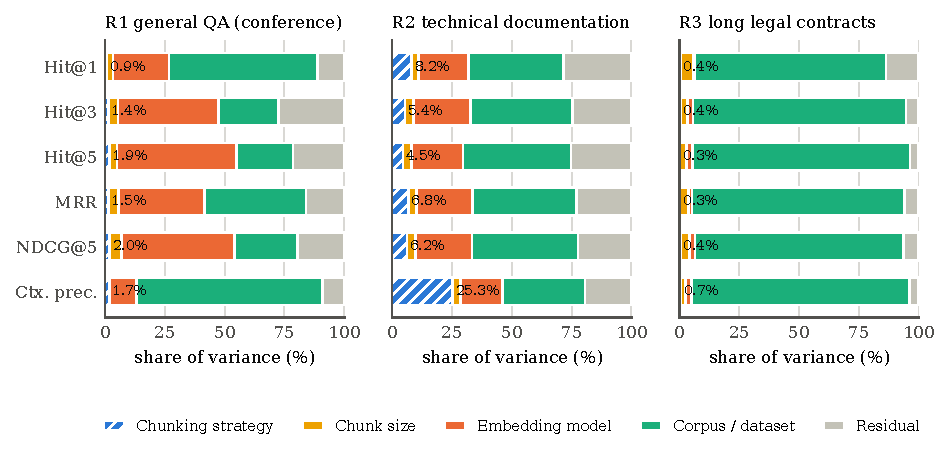
\includegraphics[width=\textwidth]{figs/fig_regimes_eta2.pdf}
\Description{Three panels of horizontal stacked bars, one per corpus regime, showing for each of six retrieval metrics how total variance divides between chunking strategy, chunk size, embedding model, corpus and residual. The chunking-strategy segment is hatched and labelled; it is 1 to 2 percent in general QA, 4.5 to 25 percent in technical documentation, and below 1 percent in legal contracts.}
\caption{Variance decomposition ($\eta^2$) per metric in the three regimes. The hatched segment is chunking strategy. R1 panel reproduced from the data of~\cite{chauhan2026chunking}, Table~1.}
\label{fig:regimes}
\end{figure}

\begin{table}[t]
\caption{Share of variance ($\eta^2$, \%) explained by chunking strategy in each regime, with 95\% bootstrap confidence intervals and Holm-corrected significance. R1 values are reproduced from Table~1 of~\cite{chauhan2026chunking}.}
\label{tab:regimes}
\centering
\small
\setlength{\tabcolsep}{4pt}
\begin{tabular}{lccc}
\toprule
Metric & R1 general QA & R2 technical docs & R3 legal contracts \\
 & ($n=32$) & ($n=576$) & ($n=96$) \\
\midrule
Hit@1 & 0.9 (n.s.) & 8.2 [6.0, 10.6]$^{***}$ & 0.4 [0.1, 2.7] (n.s.) \\
Hit@3 & 1.4 (n.s.) & 5.4 [3.6, 7.0]$^{***}$ & 0.4 [0.1, 1.4] (n.s.) \\
Hit@5 & 1.9 (n.s.) & 4.5 [3.1, 6.3]$^{***}$ & 0.3 [0.0, 0.9] (n.s.) \\
MRR & 1.5 (n.s.) & 6.8 [4.9, 8.6]$^{***}$ & 0.3 [0.0, 1.3] (n.s.) \\
NDCG@5 & 2.0 (n.s.) & 6.2 [4.4, 8.1]$^{***}$ & 0.4 [0.1, 1.5] (n.s.) \\
Context precision & 1.7 (n.s.) & 25.3 [21.0, 28.7]$^{***}$ & 0.7 [0.2, 1.6]$^{*}$ \\
\bottomrule
\end{tabular}
\\[2pt]{\footnotesize $^{***}p_{\mathrm{Holm}}<0.001$; $^{*}p_{\mathrm{Holm}}<0.05$; n.s.\ not significant.}
\end{table}


\subsection{Regime Dependence Is Statistically Robust}
\label{sec:interaction}
Pooling R2 and R3 (672 core configurations) in one model with corpus, chunk size, model and strategy main effects, the strategy-by-regime interaction explains between 12.2\% (context precision) and 19.1\% (NDCG@5) of total variance with $p<10^{-10}$ on every metric, and the finer strategy-by-corpus interaction explains 1.5--3.5\% ($p<10^{-4}$). The bootstrap intervals in Table~\ref{tab:regimes} do not overlap between R2 and R3 on any metric. After Holm correction across the six metrics, strategy is significant on all six in R2 ($p_{\mathrm{Holm}}<10^{-18}$) and on none in R3 except context precision ($p_{\mathrm{Holm}}=0.02$).

\subsection{Which Strategy Wins Depends on the Regime}
\label{sec:pairwise}
On technical documents structure-aware chunking beats every alternative (paired Cliff's $\delta$ against fixed-size $0.37$, against fixed-overlap $0.24$, against semantic $0.31$; all Wilcoxon $p<10^{-4}$, $n=144$ pairs), and fixed-overlap beats plain fixed-size ($\delta=0.16$). On contracts the generic structure-aware chunker, which here degenerates to recursive splitting, is \emph{worse} than fixed-size and fixed-overlap (paired Wilcoxon $p<0.001$ on MRR), and semantic chunking is equally poor (Table~\ref{tab:legal}).

The legal-aware parser does not change this picture. It detects section structure in 72\% of the 714 contract files (99\% of merger agreements, 85\% of non-disclosure agreements, 75\% of CUAD contracts, but only 29\% of privacy policies), so the comparison is now a genuine test of structure-aware chunking rather than of a fallback. Yet clause-aligned boundaries lower MRR relative to fixed-size windows on every sub-benchmark except MAUD, where all strategies are near zero: pooled over the 24 paired cells, the boundary effect is $-0.026$ MRR ($p=0.0006$) and adding the heading-path prefix recovers only $+0.002$ ($p=0.18$). Substituting the legal-aware chunker for the generic one in the R3 decomposition leaves chunking's share at 0.3--0.7\% (Hit@3 $p=0.04$, context precision $p=0.002$, all other metrics not significant). The most plausible reading is that contract clauses are long relative to the gold snippets (mean gold span 320--710 characters, inside sections of several thousand), so section-aligned chunks dilute the relevant sentence in more surrounding text than a fixed window does; what the heading prefix adds in topical context, the longer chunk loses in precision.

\begin{table}[t]
\caption{R3 legal contracts: mean MRR per strategy and sub-benchmark (6 cells each: 2 chunk sizes $\times$ 3 models), and the fraction of files in which the legal-aware parser detected section structure. Generic structure-aware chunking detected structure in no file and fell back to recursive splitting.}
\label{tab:legal}
\centering
\footnotesize
\setlength{\tabcolsep}{3.5pt}
\begin{tabular}{lcccccc}
\toprule
Benchmark & Fixed & Fixed-ovl. & Semantic & Struct.\ (generic) & Struct.\ (legal) & Struct.\ files \\
\midrule
PrivacyQA   & 0.505 & 0.496 & 0.447 & 0.473 & 0.470 & 29\% \\
ContractNLI & 0.235 & 0.246 & 0.234 & 0.217 & 0.195 & 85\% \\
CUAD        & 0.211 & 0.218 & 0.193 & 0.199 & 0.186 & 75\% \\
MAUD        & 0.023 & 0.027 & 0.027 & 0.022 & 0.028 & 99\% \\
\midrule
All (24 cells) & 0.243 & 0.247 & 0.225 & 0.228 & 0.220 & 72\% \\
\bottomrule
\end{tabular}
\end{table}

\subsection{What Predicts the Size of the Chunking Effect}
\label{sec:features}
\begin{figure}[t]
\centering
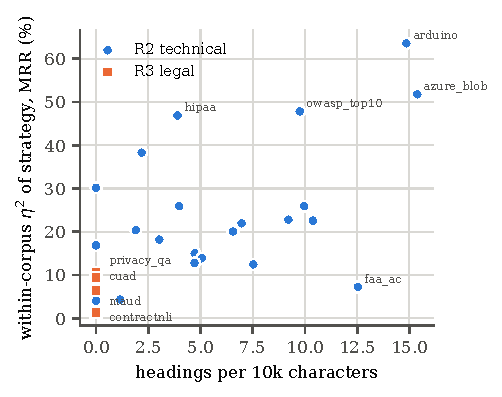
\includegraphics[width=0.62\textwidth]{figs/fig_heading_density.pdf}
\Description{Scatter plot of 28 corpora. Horizontal axis: Markdown headings per ten thousand characters, from 0 to 15. Vertical axis: within-corpus share of MRR variance explained by chunking strategy, from 0 to 65 percent. Technical documents are circles and rise with heading density; the four legal sub-benchmarks are squares clustered at zero heading density and low variance share.}
\caption{Per-corpus chunking effect against heading density for the 24 technical corpora (circles) and 4 legal sub-benchmarks (squares). Spearman $\rho=0.58$, $p=0.001$.}
\label{fig:density}
\end{figure}
For each of the 28 corpora we fit the within-corpus ANOVA (strategy, size, model; 24 cells) and regress chunking's $\eta^2$ on corpus features. Heading density (Markdown headings per 10 thousand characters) correlates with the chunking effect at Spearman $\rho=0.58$ ($p=0.001$) and with the structure-aware advantage over fixed-size at $\rho=0.72$ ($p<0.001$). Mean document length does not ($\rho=0.10$, $p=0.63$), and neither does evidence-span length ($\rho=-0.19$). In a joint linear model heading density is the only significant predictor ($p=0.002$; adjusted $R^2=0.32$); the same holds within R2 alone ($p=0.005$). Retrieval difficulty (mean Hit@5) correlates modestly with the spread between strategies ($\rho=0.44$, $p=0.02$), which we return to under the floor-effect check below. Figure~\ref{fig:density} shows the relationship.

\subsection{Floor-Effect Check for the Legal Regime}
\label{sec:floor}
Absolute span-level performance on contracts is low (mean Hit@5 0.35; 0.04 on MAUD) even though document-level Hit@5 is high (0.81--0.99): retrieval finds the right contract but not the right clause. A floor effect is therefore a competing explanation for the small $\eta^2$. We checked it three ways. Excluding MAUD raises chunking's share to 0.7--1.5\% (Hit@5 $p=0.048$); excluding both MAUD and ContractNLI, which leaves 48 cells at mean Hit@5 0.53, raises it to 1.1--2.4\% (Hit@5 $p=0.024$), reaching the general-QA level but remaining three to seven times below R2. Within PrivacyQA alone, where Hit@5 is 0.71, chunking's within-corpus share (10\%) is below the R2 median (20\%). Finally, at retrieval depths where the metric is no longer near floor, the gap persists: mean Hit@20 is 0.50 and recall@20 over gold snippets is 0.41, yet chunking explains only 0.1\% of Hit@20 variance and 0.3\% of recall@20 variance (strategy $p=0.10$ and $p=0.02$), while the sub-benchmark explains over 90\%. The regime difference thus survives the floor-effect check, although part of the R3 estimate's smallness is attributable to task difficulty, and we report R3 as ``below 1\%, and below 2.5\% under any subset we examined'' rather than as a point estimate.

\subsection{Boundaries Versus Metadata: The Prefix Ablation Replicated}
\label{sec:ablation}
Structure-aware chunkers do two things at once: they cut at structural boundaries and they prepend the heading path to each chunk. The conference paper separated the two on Natural Questions with a $2\times2$ ablation and found both effects small (boundaries $-0.034$ MRR, prefix $+0.004$). We repeat the ablation on both new regimes by adding a no-prefix variant with identical boundaries (Fig.~\ref{fig:ablation}). On technical documents (144 paired cells) both components help and both are significant: structural boundaries alone raise MRR from 0.588 to 0.634 ($+0.045$, Wilcoxon $p<10^{-13}$) and the prefix adds a further $+0.020$ ($p<10^{-7}$), so boundary placement carries about 70\% of the retrieval-stage gain. The split depends on whether structure exists: on the 30 cells from the five heading-free technical documents, the no-prefix variant (which there reduces to recursive splitting) still gains $+0.036$ over fixed-size, but the prefix adds nothing because there is no heading to prepend. On contracts with the legal-aware parser (24 paired cells) the boundary effect is negative ($-0.026$, $p<0.001$) and the prefix effect is nil ($+0.002$, $p=0.18$). Taken together with R1, the ablation yields three different answers in three regimes, which is itself the point: neither ``structure-aware chunking helps'' nor ``the gain is only metadata'' is a general statement. At the generation stage on technical documents, however, the prefix matters more than the boundaries (Sect.~\ref{sec:generation}), because the generator can use the section context directly.

\begin{figure}[t]
\centering
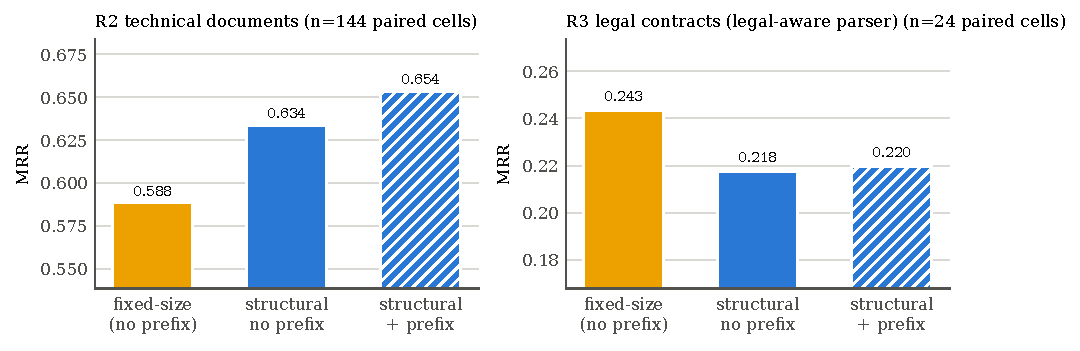
\includegraphics[width=\textwidth]{figs/fig_prefix_ablation.pdf}
\Description{Two bar charts of mean MRR for three conditions: fixed-size without prefix, structural boundaries without prefix, structural boundaries with heading prefix. Left panel, technical documents: bars rise from 0.588 to 0.634 to 0.654. Right panel, legal contracts with the legal-aware parser: bars fall from 0.244 to 0.218 and recover slightly to 0.220.}
\caption{Boundary-versus-prefix ablation on R2 technical documents (left, 144 paired cells) and R3 contracts with the legal-aware parser (right, 24 paired cells). Mean MRR; hatched bar includes the heading-path prefix.}
\label{fig:ablation}
\end{figure}

\subsection{Does Label Rigor Change the Answer?}
\label{sec:labels}
Scoring the identical R2 retrieval runs with the fuzzy word-overlap labels instead of exact spans raises every absolute metric by about seven points (MRR 0.61 to 0.68) but \emph{shrinks} chunking's share of variance, to between 63\% (Hit@5) and 89\% (Hit@1) of its span-label value, and shrinks the structure-aware advantage over fixed-size on MRR from 0.065 to 0.045. Fuzzy labels inflate fixed-size and fixed-overlap scores most (+0.076 MRR) and structure-aware least (+0.056), because loose matching credits partial overlaps that boundary-respecting chunks do not need. The correlation between the two label schemes is 0.85--0.88 per metric. Loose labels therefore blur rather than manufacture strategy differences in this regime, which cautions against reading a small chunking effect under heuristic labels as evidence that chunking is irrelevant, and equally against the conference paper's implicit assumption that heuristic labels flatter structure-aware chunking.

\subsection{Does the Technical-Regime Effect Reach the Generated Answer?}
\label{sec:generation}
The conference paper showed for R1 that chunking differences do not propagate to answer quality. We repeat that test on R2, where chunking does matter at the retrieval stage. For 200 questions sampled uniformly over the 24 technical corpora we retrieve the top five chunks under each strategy (BGE-large, 512 tokens), generate an answer with a small instruction-tuned model (Claude Haiku 4.5) from the retrieved context only, and score it with a stronger judge (Claude Opus 5) for correctness against the gold answer and faithfulness to the context, each on a 1--5 scale with a structured-output schema. Table~\ref{tab:generation} reports the results. Correctness ranges from 4.30 (semantic) to 4.53 (structure-aware) and the four core strategies do not differ significantly (Kruskal--Wallis $H=3.8$, $p=0.29$, $n=200$ per strategy); the paired structure-aware advantage over fixed-size is $+0.17$ points ($p=0.08$). Faithfulness is at ceiling (4.93--4.95) for every strategy, as in R1. Two things differ from R1. First, retrieval quality now matters for the answer: the per-question correlation between span-label MRR and correctness is $r=0.56$, against $0.28$ on Natural Questions, because technical questions are less often answerable from the generator's parametric knowledge. Second, the no-prefix variant lets us split the structure-aware gain at the generation stage: structural boundaries alone add $+0.04$ correctness over fixed-size, the heading prefix adds a further $+0.12$. The generator benefits from being told which section a passage comes from more than from where the passage was cut. Even so, the end-to-end strategy effect on technical documents is a fraction of a point on a five-point scale, and it is not statistically distinguishable from zero at $n=200$.

\begin{table}[t]
\caption{End-to-end evaluation on R2 technical documents (200 questions, top-5, BGE-large, 512 tokens). Correctness and faithfulness are 1--5 judge scores. Kruskal--Wallis across the four core strategies: correctness $p=0.29$, faithfulness $p=0.86$.}
\label{tab:generation}
\centering
\begin{tabular}{lccc}
\toprule
Strategy & MRR & Correctness & Faithfulness \\
\midrule
Fixed-size & 0.610 & 4.37 & 4.95 \\
Fixed-overlap & 0.607 & 4.42 & 4.94 \\
Semantic & 0.611 & 4.30 & 4.95 \\
Structure-aware (with prefix) & 0.629 & 4.53 & 4.95 \\
\midrule
Ablation: structure-aware, no prefix & 0.612 & 4.41 & 4.95 \\
\bottomrule
\end{tabular}
\end{table}

\subsection{Cost}
\label{sec:cost}
Chunking cost separates the strategies far more than retrieval quality does. On the technical corpora, median chunking time per document is 20\,ms for fixed-size and fixed-overlap, 139\,ms for structure-aware, and 6.7\,s for semantic chunking, which must embed every sentence before it can choose boundaries; on the contract corpora the medians are 0.8\,s, 2.7\,s, 2.7\,s and 4.6\,s per sub-benchmark for fixed-size, structure-aware, semantic and the legal-aware parser respectively, with semantic chunking's sentence-embedding pass on the 52-million-character MAUD corpus dominating the wall-clock time of the entire study. Embedding cost scales with chunk count, and structure-aware strategies produce 20--80\% more chunks than fixed-size at the same target size because sections are split at their own boundaries. Semantic chunking is therefore the only strategy that is both never best and always the most expensive, consistent with~\cite{qu2025semantic}.

\section{Discussion}
\label{sec:discussion}

\subsection{A Map, Not a Verdict}
The conference paper's claim was that chunking is a low-variance factor for QA over general-purpose corpora, and it predicted that very long documents would be the setting where that claim is most likely to fail. The three-regime map confirms the first part and refutes the second. Chunking's share of variance does not grow with document length; it peaks on medium-length, densely structured technical documentation and is smallest on the longest documents we tested. What distinguishes the regimes is not length but whether the corpus carries explicit, machine-readable structure that a chunker can exploit: heading density predicts the chunking effect across all 28 corpora, document length does not, and the five technical documents without headings behave like the legal contracts rather than like their structured neighbours. The practical reading is that chunking strategy matters exactly when there is structure to respect, and that the gain available from respecting it is bounded. Even in R2, where chunking is highly significant, its share of variance (5--8\% on ranking metrics) is a third of the embedding model's and a sixth of the corpus's. The one exception is context precision, where strategy explains a quarter of the variance in R2, because structure-aware chunks pack fewer irrelevant neighbours into the top five; this is a precision effect on the retrieved context rather than a recall effect on whether the answer is found.

This map also accounts for much of the disagreement in the recent literature. Studies that report small or inconsistent chunking effects work on general QA, academic text or source code~\cite{bennani2026systematic,caspari2026complex,kreileder2026academic,li2025enhancing}, corpora with sparse or inconsistent structural markup. Studies that report large effects work on manuals, filings, clinical guidelines and industrial documents~\cite{taiwo2026oilgas,gomezcabello2025clinical,demoura2026adaptive,jimenoyepes2024financial}, which is our R2. The clinical study's one-way $\eta^2$ of 0.11 for chunking~\cite{gomezcabello2025clinical} sits at the upper end of our R2 range once one notes that a one-way design assigns to the single factor variance that our four-factor design attributes to corpus and model. Two results remain harder to reconcile. Shaukat et al.~\cite{shaukat2026systematic} report paragraph-group chunking nearly doubling nDCG@5, but under LLM-graded relevance; our label-rigor analysis (Sect.~\ref{sec:labels}) shows that the labelling protocol changes the apparent effect size by a third even between two deterministic schemes, and graded LLM judgments are known to shift with the very context prefixes that structure-aware chunkers add~\cite{yang2026titlechain}. StrucChunk~\cite{singh2026strucchunk} doubles character recall on LegalBench-RAG, but its intervention bundles clause-aligned boundaries with cross-reference resolution and hybrid lexical--dense retrieval, and the comparison baseline is a 500-character naive splitter; our legal-aware parser isolates the boundary component and finds that clause-aligned boundaries alone \emph{lower} MRR relative to fixed windows, which suggests that StrucChunk's gain comes from the retrieval-side components of its pipeline rather than from segmentation. Neither study is wrong about its own corpus; both illustrate why absolute comparisons without variance decomposition cannot be transferred.

\subsection{Implications for Practitioners}
The heading-density result gives a diagnostic that costs nothing: count explicit section markers per ten thousand characters before running any retrieval experiment. Where that density is high (roughly above five in our corpora), a structure-aware chunker with heading prefixes is worth adopting and is the single best strategy we tested; where it is near zero, no segmentation strategy in our set recovers the difference, and the engineering budget is better spent on the embedding model, on a domain-specific structure parser, or on representation-level fixes such as contextual prefixes and late chunking~\cite{anthropic2024contextual,gunther2024latechunking,conti2025conteb}. In every regime the embedding model explains more variance than chunking strategy on every ranking metric, so model selection remains the first lever. Semantic chunking is never the best strategy in any regime and is the most expensive by one to two orders of magnitude (Sect.~\ref{sec:cost}), consistent with~\cite{qu2025semantic}. Finally, a team that evaluates a structure-aware chunker should verify that it actually detects structure on their corpus: ours silently fell back to recursive splitting on 714 contracts, and the fraction of documents in which structure is detected (reported as \texttt{structured\_files\_frac} in our results) is a cheap sanity check that benchmark reports should include.

\subsection{Implications for Benchmark Design}
The conference paper asked benchmark authors to report variance decomposition alongside absolute scores. This article adds three requests. First, report interaction terms: a main effect of chunking averaged over corpora hides the fact that the effect is concentrated in a subset of them, and the strategy-by-corpus interaction is the quantity a practitioner needs in order to know whether a published result transfers. Second, report the relevance-labelling protocol and, where feasible, score the same runs under more than one protocol; loose labels inflate absolute scores and compress strategy differences, so a benchmark that uses heuristic or LLM-graded relevance should not be read as evidence about chunking without that check. Third, characterise the corpus structurally, at minimum by heading density and document length, so that results can be placed on a map such as ours rather than treated as universal.

\subsection{Limitations}
Our map has three regimes and 30 corpora, not a continuous sampling of corpus space; the heading-density relationship is correlational and derived largely from R2, and its threshold should be treated as indicative. We tested four core strategies and two chunk sizes; proposition-level, LLM-driven and late-chunking approaches, and sizes above 512 tokens, are outside the design, as is reranking. R2 and R3 are evaluated at the retrieval stage only; the conference paper's end-to-end evaluation covered R1, and we expect, but have not shown, the same attenuation elsewhere. Absolute performance in R3 is low enough that a floor effect contributes to the small chunking share there, although the regime gap survives removal of the hardest datasets and persists at retrieval depths of 10 and 20. Each cell is a single deterministic run, so the variance decomposed is between-configuration variance; within-cell sampling variability is addressed by the bootstrap over corpora rather than by repeated runs. The legal-aware parser is a regular-expression heuristic that detects structure in 72\% of contracts (29\% of privacy policies); a learned clause segmenter might do better, although the direction of its effect where it does detect structure gives little reason to expect a reversal. All corpora are English.

\section{Conclusions}
\label{sec:conclusions}
Starting from the conference finding that chunking strategy explains 1--2\% of retrieval variance in general-purpose QA, we asked when it matters and answered with the same balanced factorial design on two further regimes and 720 new configurations. Chunking's importance is regime-dependent and non-monotonic: substantial and highly significant on structured technical documentation, negligible on general QA and on long legal contracts. The strategy-by-regime interaction, not the main effect, is the quantity that describes chunking's role, and the density of explicit document structure, not document length, predicts where that role is large. Structure-aware chunking is the right default wherever structure is machine-readable and is worse than a fixed window on long contracts, even with a domain-aware parser that finds their sections. Relevance-label rigor changes absolute scores by seven points and the measured chunking effect by a third, in the direction of blurring rather than exaggerating strategy differences. The conference paper's recommendation stands with a sharper edge: do not optimise chunking before the embedding model, but do check your corpus for structure first, because that is where the remaining chunking gain lives. Benchmarks that report variance decomposition, interaction terms, the labelling protocol and corpus structure would let the community stop relitigating whether chunking matters and start saying where.

\begin{credits}
\subsubsection{\ackname}
Code, the technical-document corpus with its question--answer pairs, and all per-configuration results are available at \url{https://github.com/aadityc91/TechChunkBench} (branch \texttt{ccis-extension}). LegalBench-RAG was obtained from its authors' public release~\cite{pipitone2024legalbenchrag} and is not redistributed.

\subsubsection{Disclosure of Interests}
The authors have no competing interests to declare that are relevant to the content of this article.

\subsubsection{Disclosure of AI Use}
The manuscript, or parts thereof, was drafted and edited with the assistance of artificial intelligence (AI) using Claude developed by Anthropic (Claude Fable 5.1, November 2026), based on the authors' experimental design, results and interpretations. Experiment code and analysis scripts used within this manuscript were written and refined with the assistance of the same tool. The generated content was carefully reviewed, verified and endorsed by the authors to ensure the accuracy and integrity of the final manuscript.
\end{credits}

\bibliographystyle{splncs04}
\bibliography{references}

\end{document}
